\section{Results}
\label{sec:results}

The analytic cohort feeds $179{,}141$ training samples (one per admission
per training-eligible window), $4{,}600$ validation admissions and
$4{,}686$ held-out test admissions, split by patient. Every reported
number in this section is at $K_{\mathrm{eval}} = 4$ days with a label
horizon of $(96, 336]$ hours. Confidence intervals are $2{,}000$-resample
patient-level bootstraps.

\subsection{Target support}
\label{sec:results-support}

\begin{figure}[htbp]
\centering
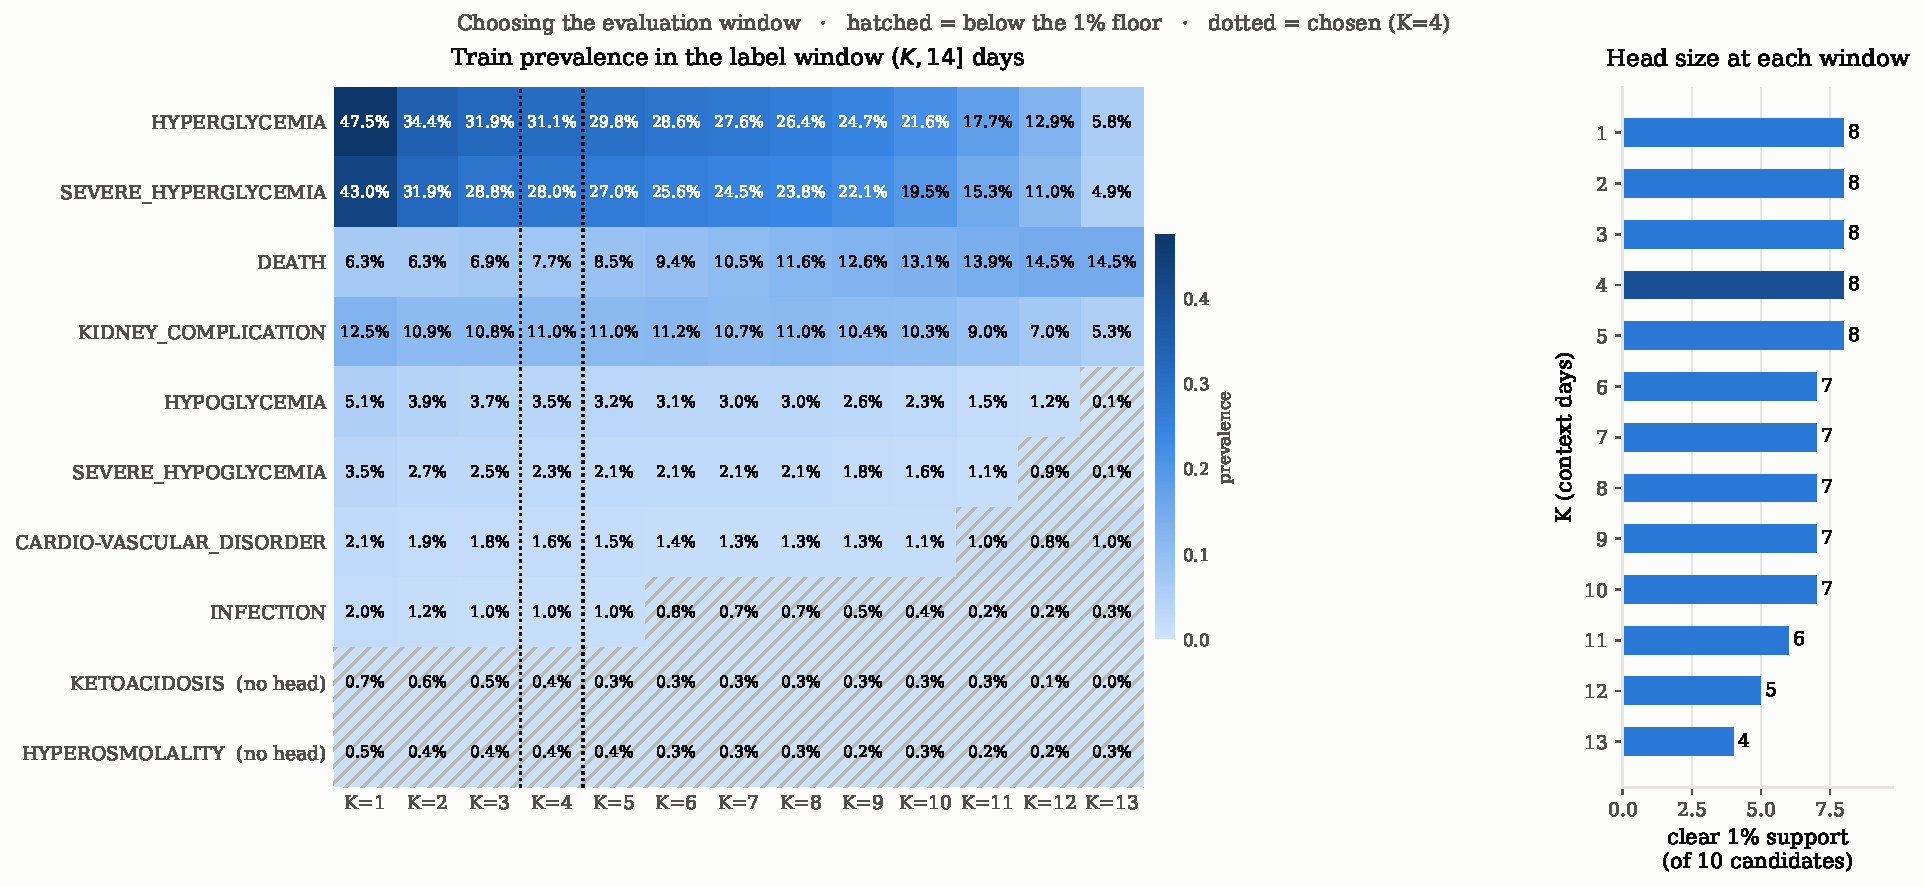
\includegraphics[width=\textwidth]{fig1_target_support}
\caption{Target support across candidate context windows on the Kineret
cohort. Prevalence is per admission on the training split; each candidate
target's line traces its prevalence as $K$ moves from $1$ to $13$ days.
The horizontal line at $1\%$ is the prevalence threshold; targets below
it at $K_{\mathrm{eval}}$ do not receive a prediction head.}
\label{fig:target-support}
\end{figure}

Figure~\ref{fig:target-support} shows the eight retained targets at
$K = 4$: hyperglycemia ($n_+ = 1{,}470$), severe hyperglycemia
($1{,}317$), kidney complication / AKI ($566$), $30$-day mortality
($341$), hypoglycemia ($181$), severe hypoglycemia ($111$), MI /
cardiovascular ($69$), and infection ($37$). Hyperosmolality
($n_+ \approx 220$, prevalence $\approx 0.44\%$) and ketoacidosis
($n_+ \approx 330$, $\approx 0.66\%$) fall below the $1\%$ threshold at
$K = 4$ and do not receive heads. Both would clear the threshold at
$K = 1$, but were excluded to hold the head layout fixed at the chosen
evaluation window; a target that flickers in and out of the head list
across arms would not admit a clean cross-arm comparison. Choosing the
window from this table before training keeps the results a single
support-conditioned table rather than a surface over $K$.

\subsection{The ladder}
\label{sec:results-ladder}

\begin{figure}[htbp]
\centering
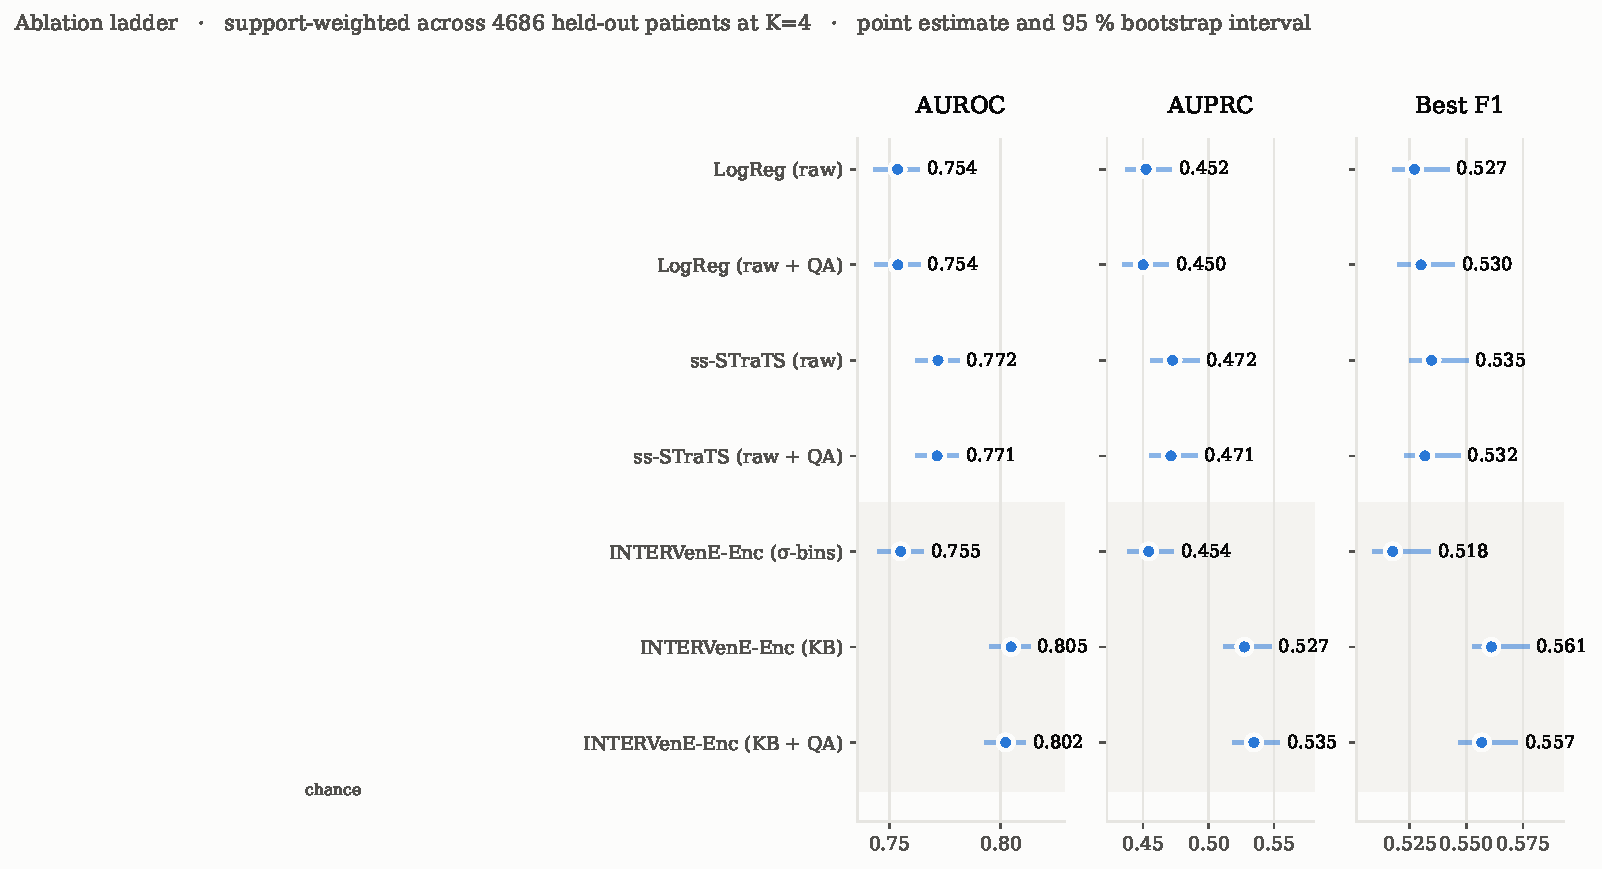
\includegraphics[width=\textwidth]{fig2_ladder}
\caption{Support-weighted performance across the seven arms on
$4{,}686$ held-out test admissions at $K = 4$, with $95\%$ patient-level
bootstrap intervals ($2{,}000$ resamples). Rungs $5\to 6$ isolate the
knowledge base; $6 \to 7$ the treatment-quality signal.}
\label{fig:ladder}
\end{figure}

\begin{table}[htbp]
\centering
\small
\caption{Support-weighted performance across the seven arms at $K = 4$.
Bold marks the best value in each column; brackets are $95\%$
patient-level bootstrap intervals.}
\label{tab:ladder}
\begin{tabular}{clccccc}
\toprule
Rung & Arm & AUROC & AUPRC & Best $F_1$ & Onset MAE (h) & LoS MAE (h) \\
\midrule
1 & LogReg                       & $0.754$ [$0.743,0.764$] & $0.452$ [$0.436,0.472$] & $0.527$          & $32.9$ & $47.7$ \\
2 & LogReg $+$ QA                & $0.754$ [$0.743,0.764$] & $0.450$ [$0.434,0.469$] & $0.530$          & $33.1$ & $47.7$ \\
3 & ss-STraTS                    & $0.772$ [$0.762,0.781$] & $0.472$ [$0.456,0.493$] & $0.535$          & $33.2$ & $46.4$ \\
4 & ss-STraTS $+$ QA             & $0.771$ [$0.762,0.781$] & $0.471$ [$0.455,0.491$] & $0.532$          & $32.8$ & $47.7$ \\
5 & INTERVenE-Enc ($\sigma$-bins)& $0.755$ [$0.744,0.765$] & $0.454$ [$0.438,0.473$] & $0.518$          & $33.3$ & $\mathbf{45.1}$ \\
6 & \textbf{INTERVenE-Enc (KB)}  & $\mathbf{0.805}$ [$0.795,0.813$] & $0.527$ [$0.511,0.548$] & $\mathbf{0.561}$ & $\mathbf{30.8}$ & $45.9$ \\
7 & INTERVenE-Enc (KB $+$ QA)    & $0.802$ [$0.793,0.811$] & $\mathbf{0.535}$ [$0.518,0.554$] & $0.557$ & $30.9$ & $46.0$ \\
\bottomrule
\end{tabular}
\end{table}

The architecture transfers. INTERVenE-Enc on knowledge-based
abstractions leads every arm on AUROC, best $F_1$ and onset error, at a
support-weighted AUPRC of $0.527$ against $0.472$ for the best
raw-stream baseline (ss-STraTS), with non-overlapping bootstrap
intervals (Table~\ref{tab:ladder}, Figure~\ref{fig:ladder}). The
KB $+$ QA arm edges KB alone on AUPRC ($0.535$ vs $0.527$), separated
by less than one interval width; the QA delta is decomposed in
Section~\ref{sec:results-qa}.

\paragraph{The knowledge base is doing predictive work.}
Replacing KBTA with $\sigma$-bin discretization (rung $5$) costs $0.073$
AUPRC and $0.050$ AUROC relative to rung $6$, and drops the arm to the
logistic-regression floor. The same substitution on MIMIC-IV
\citep{oded2027intervene} was within noise---the ablation there
attributed accuracy on that cohort to the Transformer over persistent
intervals rather than to the semantic content of the intervals. On the
data the knowledge base was authored for, that no longer holds:
clinical knowledge is doing predictive work, not only interpretive
work.

\paragraph{The architecture matters beyond having intervals.}
The floor is comfortably above chance ($0.754$ AUROC, $0.452$ AUPRC),
and ss-STraTS lifts AUROC and AUPRC only modestly over it ($+0.018$
AUROC, $+0.020$ AUPRC, both intervals overlapping the LogReg CI at the
lower end). The dominant modelling gain in the ladder is $6-3$: the
Transformer over KBTA intervals over the Transformer over triplets
($+0.033$ AUROC, $+0.055$ AUPRC, non-overlapping). Rungs $5-3$, which
compares the same INTERVenE-Enc architecture on $\sigma$-bins against
ss-STraTS on the raw stream, is within noise---the interval-based
Transformer is not intrinsically stronger, it becomes so once the
intervals carry named clinical concepts.

\paragraph{Length of stay.}
The $\sigma$-bin arm has the lowest length-of-stay error ($45.1$\,h),
below both KB arms ($45.9$--$46.0$\,h) and the raw-data arms
($46.4$--$47.7$\,h). Onset and length-of-stay heads share only the
encoder; the $\sigma$-bin encoder yields a marginally better LoS
signal despite the weakest risk performance. Onset is where the KB
arms separate cleanly: $30.8$\,h vs $32.9$--$33.3$\,h for every
raw-stream and $\sigma$-bin arm, a $\sim 2$\,h tightening that
survives bootstrap.

\subsection{The quality-assessment signal}
\label{sec:results-qa}

\begin{figure}[htbp]
\centering
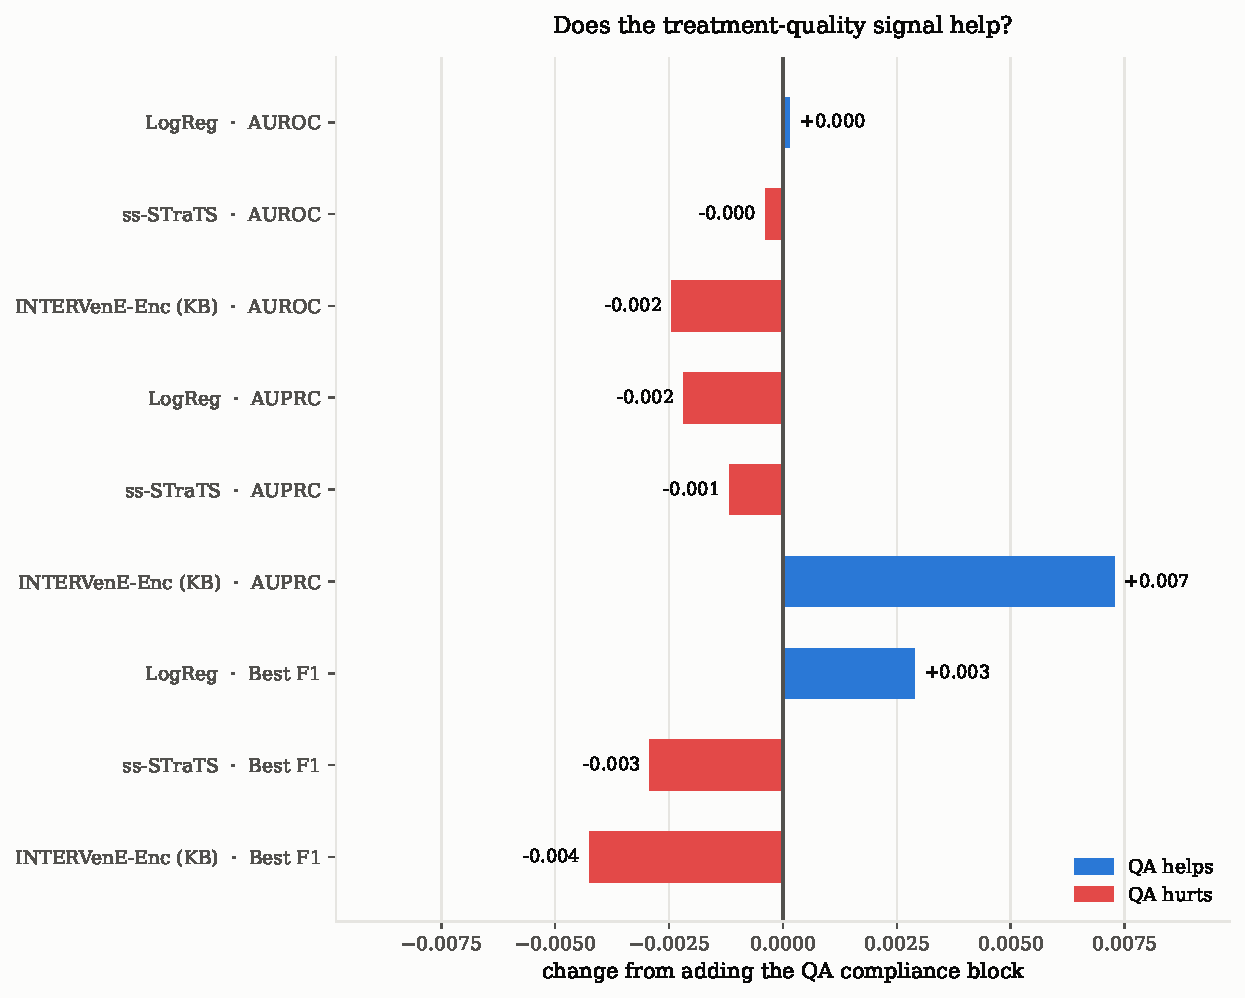
\includegraphics[width=0.85\textwidth]{fig3_qa_delta}
\caption{Change in support-weighted metrics from adding the aggregated
QA compliance block, per model. Positive values favour QA; error bars
are $95\%$ bootstrap intervals for the delta.}
\label{fig:qa-delta}
\end{figure}

Not measurably in aggregate. Every change sits at the third decimal
place with overlapping intervals (Figure~\ref{fig:qa-delta}). The
largest single change is INTERVenE-Enc's $+0.007$ AUPRC, and it is the
only arm that receives the compliance patterns as temporal tokens
rather than only as context.

The model \emph{does} use them. Sparse-transcoder attribution on the
QA arm, following the pipeline of \citep{oded2027intervene}, puts
\texttt{*\_PATTERN} tokens among the top drivers for seven of the
eight outcomes on this cohort: routine glucose monitoring for death
and kidney complication, basal-dosage and metformin-continuation
patterns for the glycemic endpoints, and reduced basal insulin after
hypoglycemia for severe hypoglycemia (attribution figure reproduced
from the concurrent methodological analysis; not shown here to
preserve the AIIM figure budget---see~\TODO{figure decision}). The
signal is read and assigned weight; it simply does not change the
aggregate metrics.

The interpretation is straightforward. The QA scores are derived
deterministically by the same abstraction engine that emits the
intervals the model is already reading; a model that reads
\emph{Glucose measured at $t$, insulin administered at $t + \delta$}
is close to computing \emph{compliance with insulin-following-
hyperglycemia at $t$} itself. The added signal is available and
used, but carries little the interval stream does not.

\subsection{Per-outcome results}
\label{sec:results-per-target}

\begin{figure}[htbp]
\centering
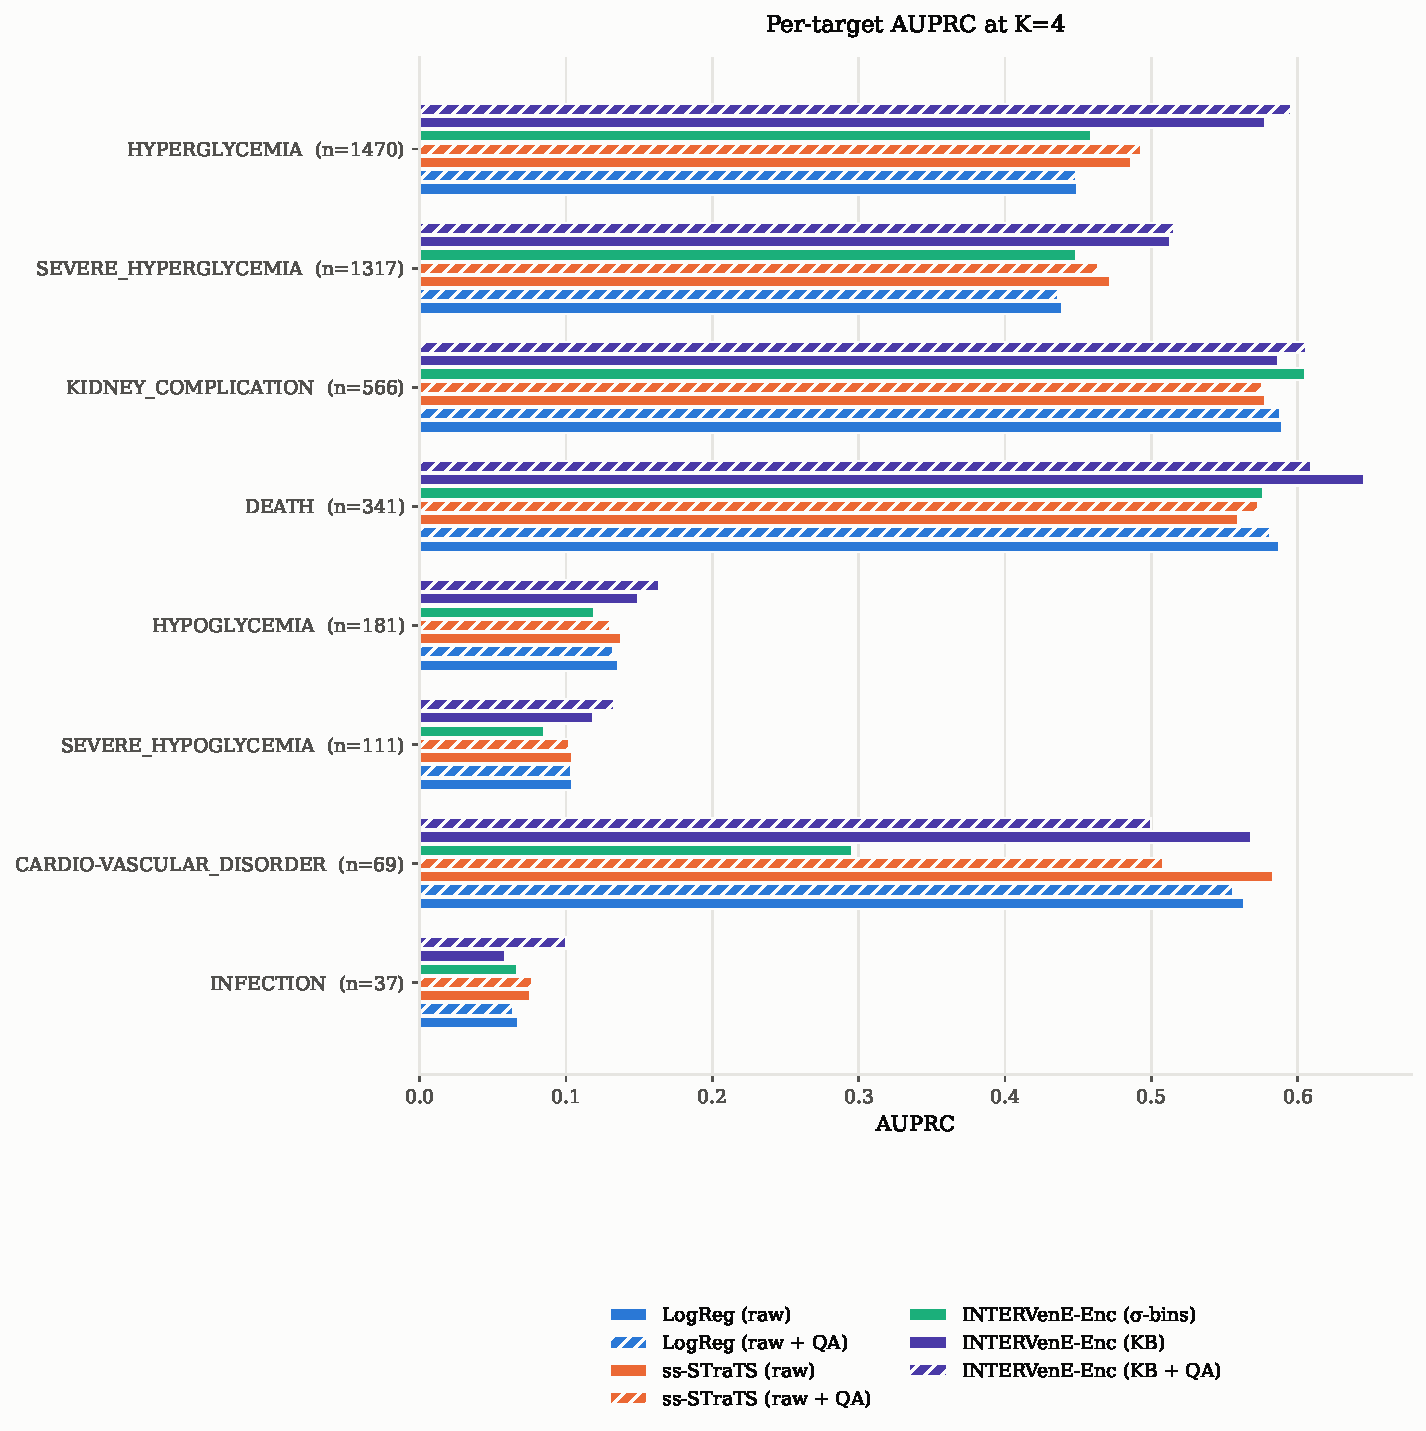
\includegraphics[width=\textwidth]{fig4_per_target_auprc}
\caption{Per-outcome AUPRC across the seven arms, ordered left-to-right
by positive count on the test set (dashed grey line: outcome
prevalence, the AUPRC random baseline).}
\label{fig:per-target-auprc}
\end{figure}

\begin{table}[htbp]
\centering
\small
\caption{Per-outcome AUPRC at $K = 4$, ordered by positive count. LR is
logistic regression, ST is ss-STraTS, $\sigma$ is INTERVenE-Enc on
$\sigma$-bins, KB and KB$+$QA the knowledge-based arms. Bold marks the
best value in each row; AKI is acute kidney injury; MI, myocardial
infarction.}
\label{tab:per-outcome}
\begin{tabular}{lrccccccc}
\toprule
Outcome & $n_+$ & LR & LR+QA & ST & ST+QA & $\sigma$ & KB & KB+QA \\
\midrule
Hyperglycemia         & 1{,}470 & 0.450 & 0.449 & 0.486 & 0.493 & 0.459 & 0.578 & \textbf{0.595} \\
Severe hyperglycemia  & 1{,}317 & 0.439 & 0.436 & 0.472 & 0.463 & 0.449 & 0.513 & \textbf{0.516} \\
AKI / kidney compl.   &   566   & 0.590 & 0.588 & 0.578 & 0.576 & 0.605 & 0.587 & \textbf{0.606} \\
Death                 &   341   & 0.587 & 0.581 & 0.559 & 0.573 & 0.577 & \textbf{0.645} & 0.609 \\
Hypoglycemia          &   181   & 0.135 & 0.132 & 0.138 & 0.130 & 0.119 & 0.149 & \textbf{0.163} \\
Severe hypoglycemia   &   111   & 0.104 & 0.103 & 0.104 & 0.102 & 0.085 & 0.119 & \textbf{0.133} \\
MI / cardiovascular   &    69   & 0.564 & 0.556 & \textbf{0.583} & 0.508 & 0.295 & 0.568 & 0.500 \\
Infection             &    37   & 0.067 & 0.064 & 0.076 & 0.077 & 0.067 & 0.058 & \textbf{0.100} \\
\bottomrule
\end{tabular}
\end{table}

The aggregate ordering is carried by the two frequent glycemic outcomes,
where the knowledge-based arms gain most: hyperglycemia $0.578$ against
$0.486$ for ss-STraTS, severe hyperglycemia $0.513$ against $0.472$.
Death is the only outcome where KB without QA leads outright ($0.645$).
Hyperglycemia is a lab-threshold event by definition; the KB collapses
$100$-plus glucose lab codes and $10$-plus insulin drugs into a single
\emph{glucose-state} and a single \emph{basal-insulin-context} channel,
and the model reads the abstraction directly. For death, no single
threshold defines the outcome, and the lift ($+0.086$ over ss-STraTS)
suggests the model is composing evidence across several
abstracted states.

Below roughly $200$ positives, the arms stop separating. Infection ($37$
positives), MI/cardiovascular ($69$) and severe hypoglycemia ($111$)
sit near their prevalence floors throughout, and the single largest
swing in the table---the $\sigma$-bin arm at $0.295$ on MI/cardiovascular
against $0.564$ for logistic regression---rests on $69$ events and
should not be read as an ordering. Weighting all eight outcomes equally
rather than by support lowers every figure (macro AUPRC $0.332$ to
$0.403$) but leaves the ranking of the arms unchanged.

\subsection{Onset and length of stay}

\begin{figure}[htbp]
\centering
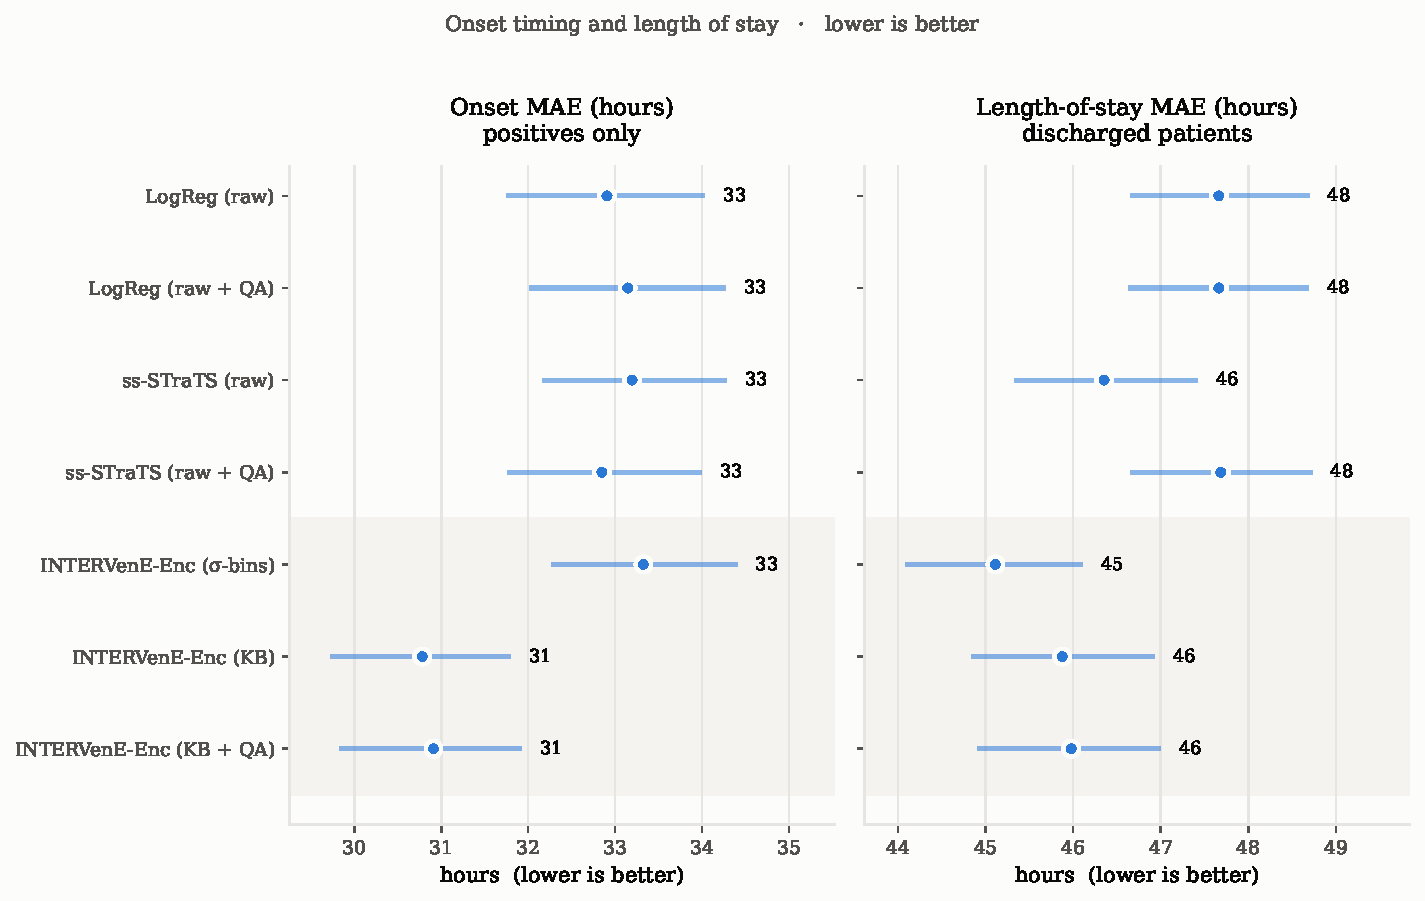
\includegraphics[width=\textwidth]{fig5_onset_and_los}
\caption{Onset MAE (hours, positives only) and length-of-stay MAE
(hours) per arm at $K = 4$. Onset is aggregated across outcomes by
support weighting; length of stay is a single regression head.
Error bars are $95\%$ bootstrap intervals.}
\label{fig:onset-los}
\end{figure}

Onset error tightens by $\sim 2$\,hours for the KB arms ($30.8$--$30.9$\,h)
relative to the raw-stream and $\sigma$-bin arms ($32.9$--$33.3$\,h;
Figure~\ref{fig:onset-los}). Length of stay error is close across the
ladder ($45.1$--$47.7$\,h), and does not track risk performance: the
$\sigma$-bin arm has the lowest LoS despite the weakest risk metrics,
because the two heads share only the encoder. The KB arms $6$ and $7$
sit essentially on top of one another for both time heads, consistent
with QA leaving aggregate metrics untouched.
